\documentclass[15pt, mathserif]{beamer}

\usepackage[french]{babel}
\usepackage[T1]{fontenc}
\usepackage[utf8]{inputenc}
%\usepackage{esvect}
\usepackage{bm}
\usepackage{eurosym}
\usepackage{tikz}
\usepackage{pgf,tikz,pgfplots}
\pgfplotsset{compat=1.15}
\usepackage{mathrsfs}
\usetikzlibrary{arrows}
\usetikzlibrary{arrows.meta}

\usetikzlibrary{mindmap}
\usepackage{multicol}
\usepackage[tikz]{bclogo}
\usepackage{tkz-tab}
\usepackage{amsmath, tabu}
\usepackage{esvect} %\vv{AB} pour le vecteur AB

\DeclareMathOperator{\e}{e}

%% Tableau

\usepackage{makecell}
\setcellgapes{1pt}
\makegapedcells
\newcolumntype{R}[1]{>{\raggedleft\arraybackslash }b{#1}}
\newcolumntype{L}[1]{>{\raggedright\arraybackslash }b{#1}}
\newcolumntype{C}[1]{>{\centering\arraybackslash }b{#1}}


%pour avoir des parenthèses rondes dans le package fourier
\DeclareSymbolFont{cmoperators}   {OT1}{cmr} {m}{n}
\DeclareSymbolFont{cmlargesymbols}{OMX}{cmex}{m}{n}

\usefonttheme{professionalfonts} %permet d'enlever un bug avec fourier
\usepackage{fourier}
\DeclareMathDelimiter{(}{\mathopen} {cmoperators}{"28}{cmlargesymbols}{"00}
\DeclareMathDelimiter{)}{\mathclose}{cmoperators}{"29}{cmlargesymbols}{"01}

%Graphiques 

\usepackage{pgf,tikz,pgfplots}
\pgfplotsset{compat=1.15}
\usepackage{mathrsfs}
\usetikzlibrary{arrows}
\usetikzlibrary{mindmap}

%ensembles de nbres

\newcommand{\R}{\mathbb{R}}			%permet d'écrire le R "ensemble des réels"'
\newcommand{\N}{\mathbb{N}}			%permet d'écrire le N "ensemble des entiers naturels"
\newcommand{\Z}{\mathbb{Z}}			%permet d'écrire le Z "ensemble des entiers relatifs"
\newcommand{\Prem}{\mathbb{P}}	%permet d'écrire le P "ensemble des nombres premiers" (qui n'a pas marché avec le \P car il existe déjà)
\newcommand{\D}{\mathbb{D}}
\newcommand{\Df}{\mathcal{D}_f}
\newcommand{\Cf}{\mathcal{C}_f}

\newcommand{\Q}{\mathbb{Q}}


\newcommand{\st}[1]{$(#1_n)_{n \in \N}$}

\usetheme{Madrid}
\useoutertheme{miniframes} % Alternatively: miniframes, infolines, split
\useinnertheme{circles}
\definecolor{UBCblue}{rgb}{0.1, 0.25, 0.4} % UBC Blue (primary)
\definecolor{bordeaux}{RGB}{128,0,0}
\usecolortheme[named=UBCblue]{structure}

\usepackage{color} % J'aime bien définir mes couleurs
\definecolor{propcolor}{rgb}{0, 0.5, 1}
\definecolor{thcolor}{rgb}{0.6, 0.07, 0.07}
\colorlet{louis}{blue!70!green!60!white}
\colorlet{sakura}{pink!40!red}

\title{Activités Mentales}
\date{24 Août 2023}

\newcommand{\vco}[2]{\begin{pmatrix} #1 \\ #2 \end{pmatrix}} %Coordonnées de vecteur
\newenvironment{eq}{\begin{cases}\begin{tabu}{ccccc}}{\end{tabu}\end{cases}}
\newenvironment{eql}{\begin{cases}\begin{tabu}{cccccl}}{\end{tabu}\end{cases}}
\newenvironment{eqrl}{\begin{cases}\begin{tabu}{rl}}{\end{tabu}\end{cases}}

\newenvironment{Eq}{\begin{center}\begin{tabular}{rrcl}}{\end{tabular}\end{center}}
\newcommand{\ligneq}[2]{$\Longleftrightarrow$ & $#1$ & $=$ & $#2$ \\}
\newcommand{\Ligneq}[2]{ & $#1$ & $=$ & $#2$ \\}

\newenvironment{RPN}{\begin{center}\begin{tabular}{rrclcrcl}}{\end{tabular}\end{center}}
\newcommand{\Lignerpn}[4]{ & $#1$ & $=$ & $#2$ & ou & $#3$ & $=$ & $#4$ \\}
\newcommand{\lignerpn}[4]{$\Longleftrightarrow$ & $#1$ & $=$ & $#2$ & ou & $#3$ & $=$ & $#4$ \\}

\newenvironment{TRPN}{\begin{center}\begin{tabular}{rrclcrclcrcl}}{\end{tabular}\end{center}}
\newcommand{\Lignetrpn}[6]{ & $#1$ & $=$ & $#2$ & ou & $#3$ & $=$ & $#4$ & ou & $#5$ & $=$ & $#6$ \\}
\newcommand{\lignetrpn}[6]{$\Longleftrightarrow$ & $#1$ & $=$ & $#2$ & ou & $#3$ & $=$ & $#4$ & ou & $#5$ & $=$ & $#6$ \\}
\begin{document}

\begin{frame}
    \titlepage
\end{frame}

\begin{frame} 
	\frametitle{Question 1}
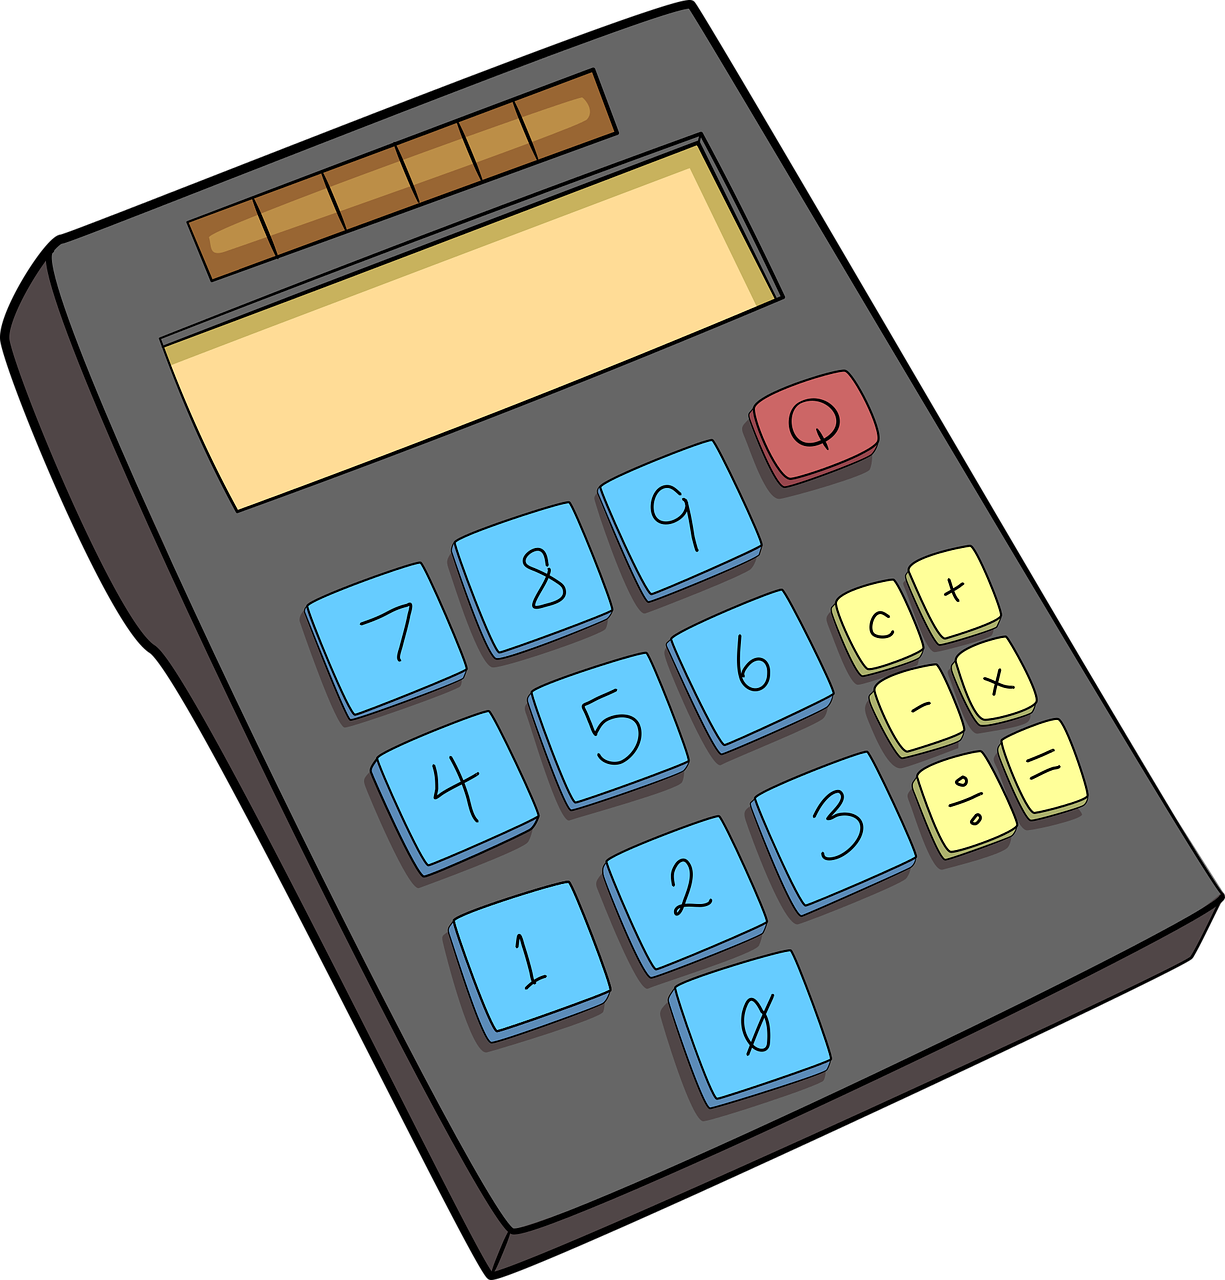
\includegraphics[scale=0.01]{calculatrice} Lors d'un congrès, 68\% des participants parlent anglais et parmi eux, 21\% ont déjà visité l'Angleterre. \\ Donner le pourcentage d'anglophone ayant déjà visité l'Angleterre.\end{frame}


\begin{frame} 
	\frametitle{Question 2}
 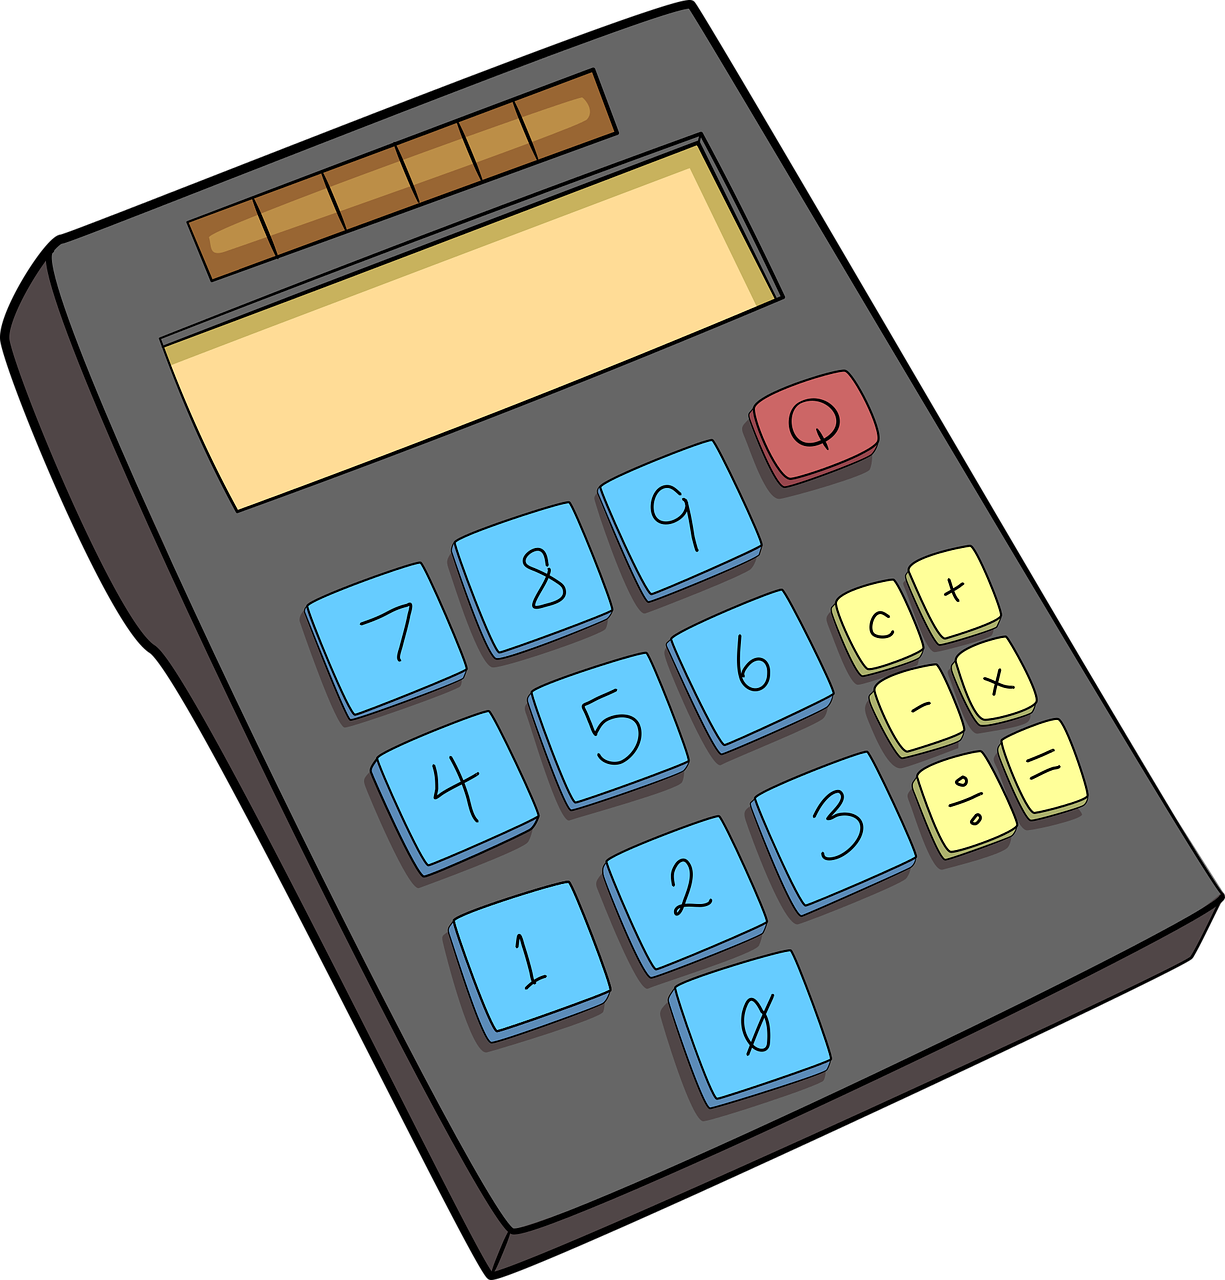
\includegraphics[scale=0.01]{calculatrice} Dans un magasin, 31 \% des articles sont des pantalons. Parmi les pantalons, 74 \% sont pour les filles. \\ Quelle est la proportion des pantalons pour fille parmi l'ensemble des articles du magasin ?\end{frame}


\begin{frame} 
	\frametitle{Question 3}
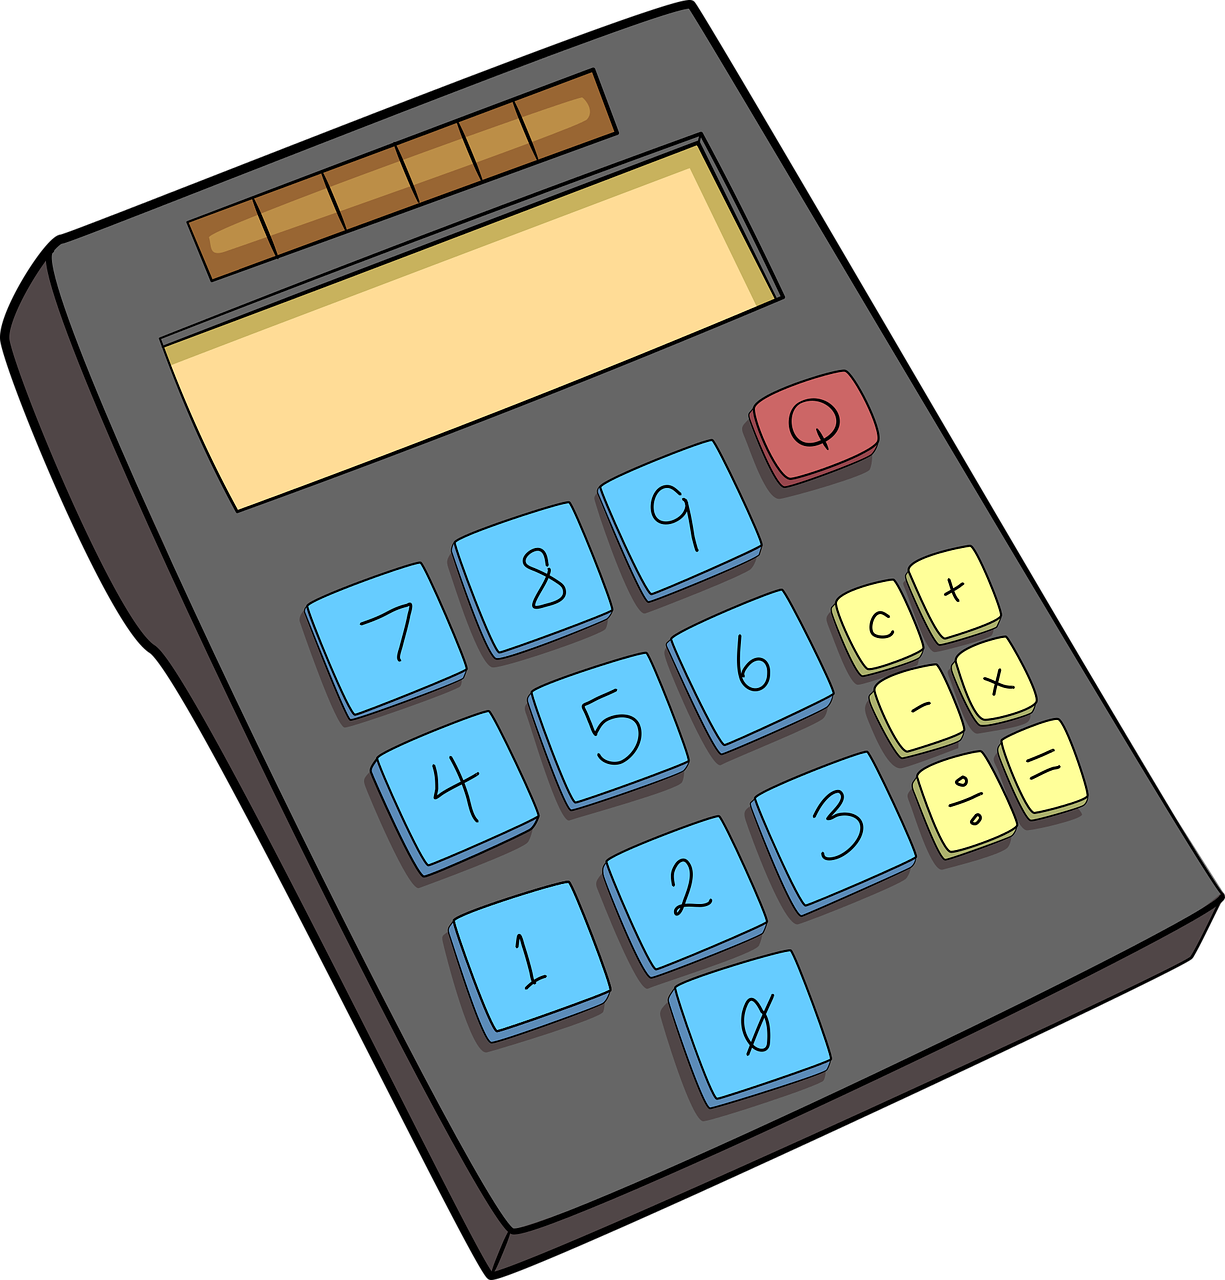
\includegraphics[scale=0.01]{calculatrice} Dans une confiserie, 28 \% des bonbons sont des sucettes. Parmi les sucettes, 37\% sont à l'anis. \\ Quelle est la proportion des sucettes à l'anis parmi l'ensemble des bonbons de la confiserie ?\end{frame}


\begin{frame} 
	\frametitle{Question 4}
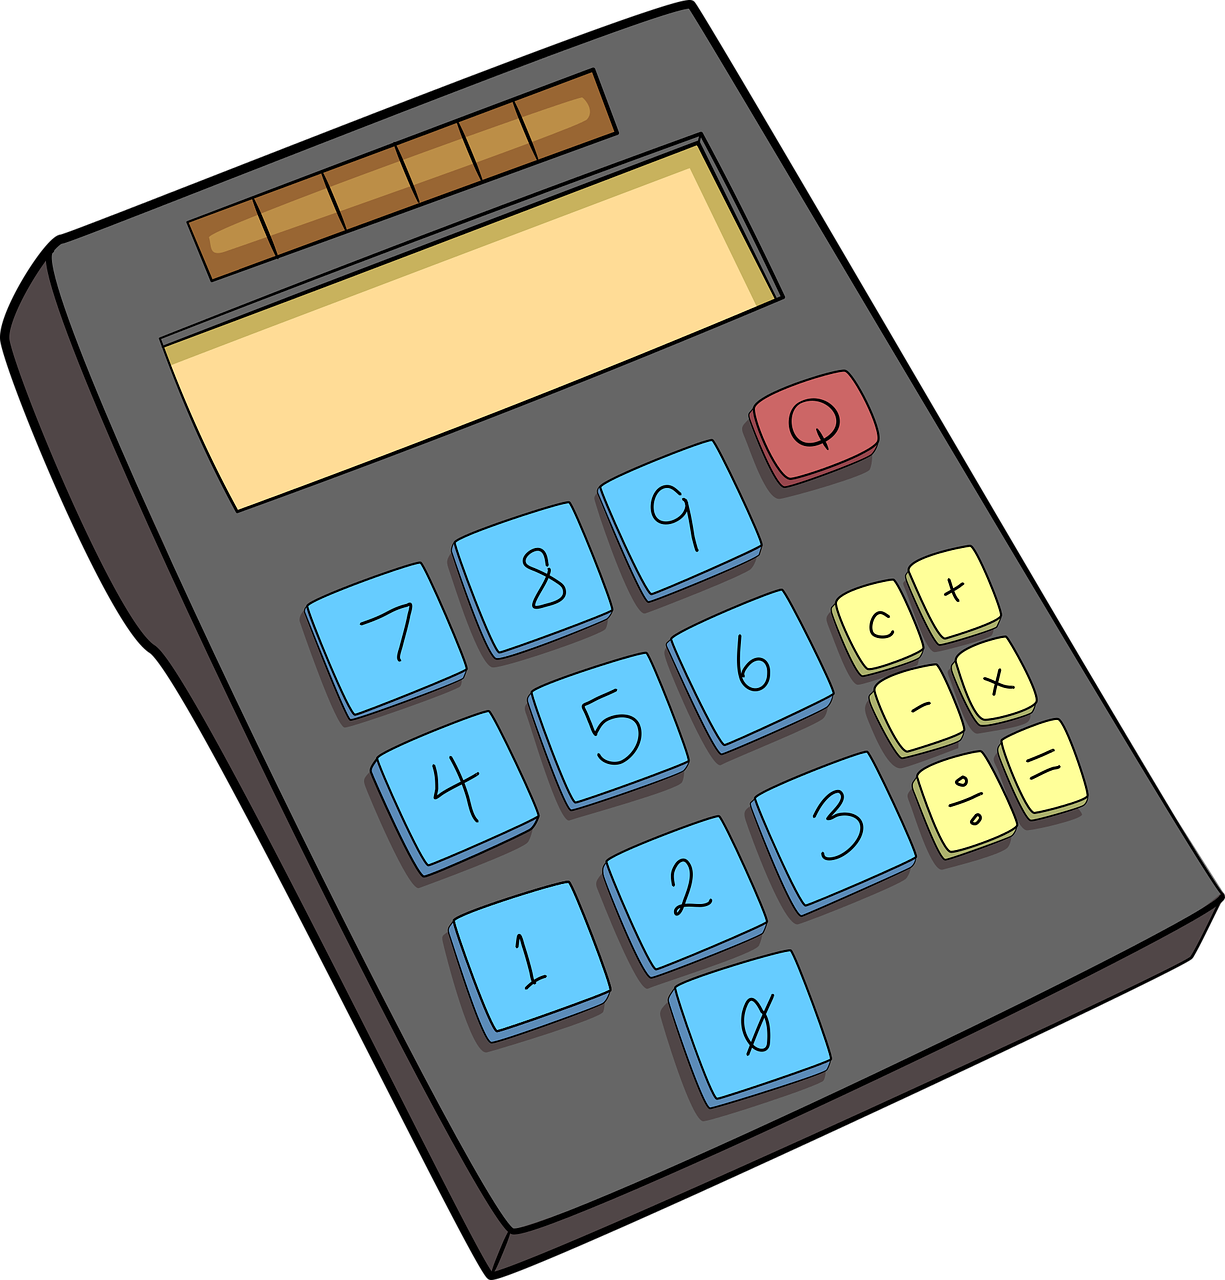
\includegraphics[scale=0.01]{calculatrice} Dans une confiserie, 40 \% des bonbons sont des sucettes. Parmi les sucettes, 16\% sont à l'anis. \\ Quelle est la proportion des sucettes à l'anis parmi l'ensemble des bonbons de la confiserie ?\end{frame}


\begin{frame} 
	\frametitle{Question 5}
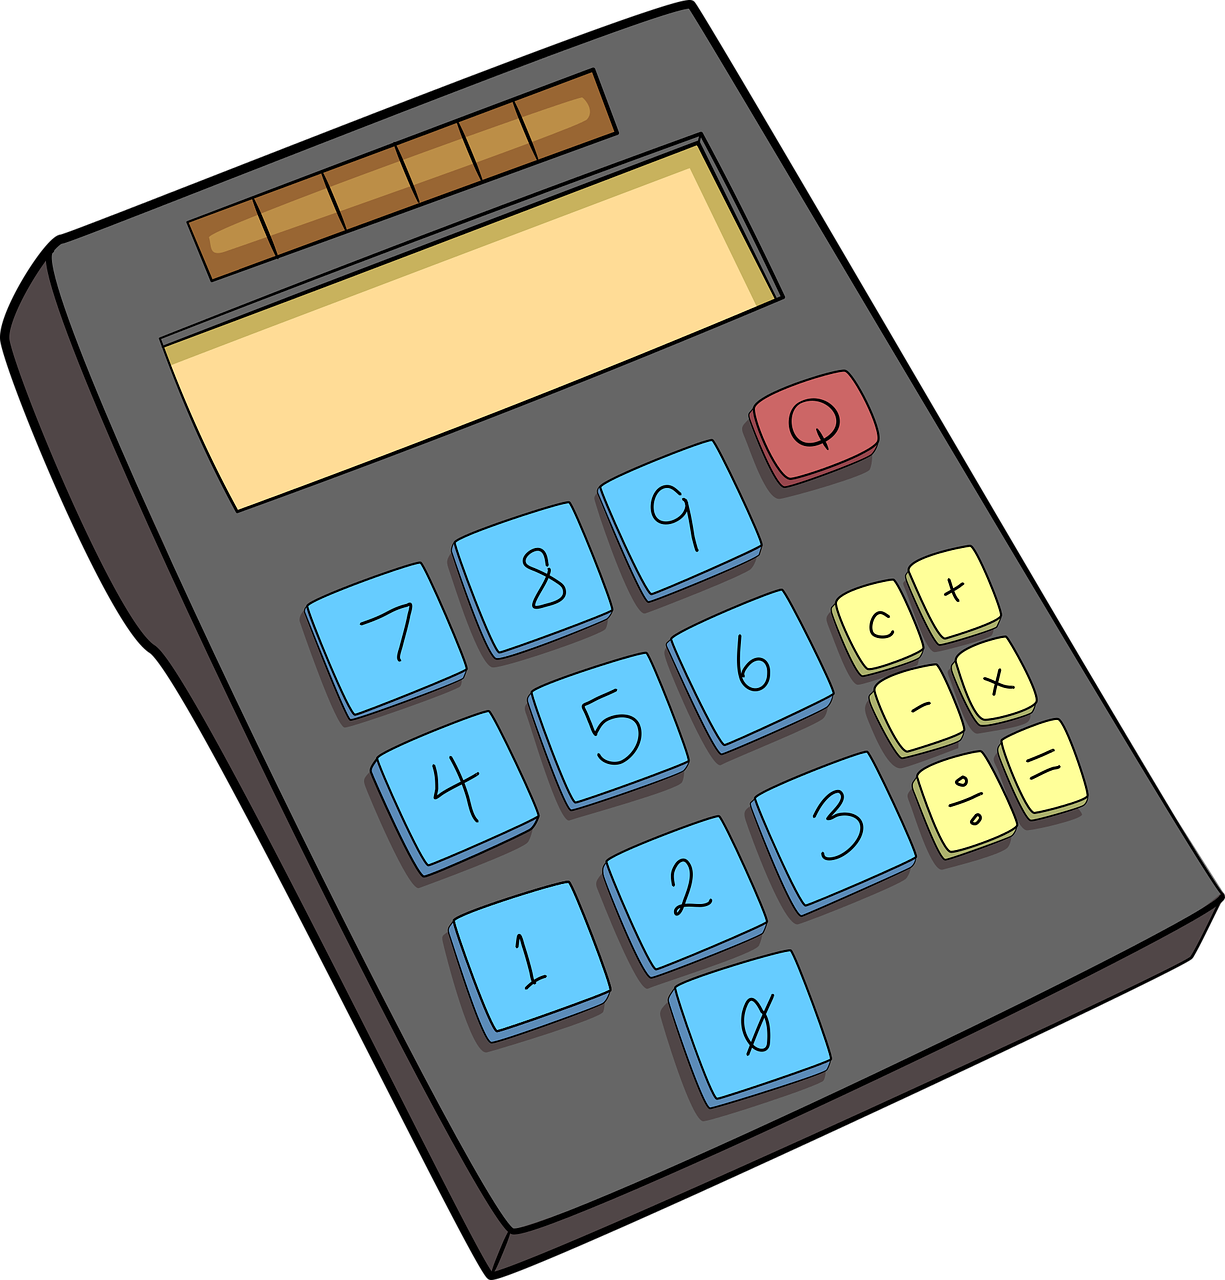
\includegraphics[scale=0.01]{calculatrice} Dans une confiserie, 47 \% des bonbons sont des sucettes. Parmi les sucettes, 56\% sont à l'anis. \\ Quelle est la proportion des sucettes à l'anis parmi l'ensemble des bonbons de la confiserie ?\end{frame}


\begin{frame}
\vspace{-10mm}
	\frametitle{Correction 1}
Lors d'un congrès, 68\% des participants parlent anglais et parmi eux, 21\% ont déjà visité l'Angleterre. Donner le pourcentage d'anglophone ayant déjà visité l'Angleterre. \\ On doit ici calculer une proportion de proportion : On doit donc multiplier les deux proportions $$ \dfrac{68}{100} \times \dfrac{21}{100} = \dfrac{1428}{10000} = 0.1428$$ Ainsi, la proportion d'anglophone ayant déjà visité l'Angleterre est de 14.28\% .\end{frame}


\begin{frame}
\vspace{-10mm}
	\frametitle{Correction 2}
Dans un magasin, 31 \% des articles sont des pantalons. Parmi les pantalons, 74 \% sont pour les filles. Quelle est la proportion des pantalons pour fille parmi l'ensemble des articles du magasin ? \\ On doit ici calculer une proportion de proportion : On doit donc multiplier les deux proportions $$ \dfrac{31}{100} \times \dfrac{74}{100} = \dfrac{2294}{10000} = 0.2294$$ Ainsi, la proportion des pantalons pour fille parmi l'ensemble des articles du magasin  est de 22.94\% .\end{frame}


\begin{frame}
\vspace{-10mm}
	\frametitle{Correction 3}
Dans une confiserie, 28 \% des bonbons sont des sucettes. Parmi les sucettes, 37\% sont à l'anis. Quelle est la proportion des sucettes à l'anis parmi l'ensemble des bonbons de la confiserie ?\\ On doit ici calculer une proportion de proportion : On doit donc multiplier les deux proportions $$ \dfrac{28}{100} \times \dfrac{37}{100} = \dfrac{1036}{10000} = 0.1036$$ Ainsi, la proportion des sucettes à l'anis parmi l'ensemble des bonbons de la confiserie  est de 10.36\% .\end{frame}


\begin{frame}
\vspace{-10mm}
	\frametitle{Correction 4}
Dans une confiserie, 40 \% des bonbons sont des sucettes. Parmi les sucettes, 16\% sont à l'anis. Quelle est la proportion des sucettes à l'anis parmi l'ensemble des bonbons de la confiserie ?\\ On doit ici calculer une proportion de proportion : On doit donc multiplier les deux proportions $$ \dfrac{40}{100} \times \dfrac{16}{100} = \dfrac{640}{10000} = 0.064$$ Ainsi, la proportion des sucettes à l'anis parmi l'ensemble des bonbons de la confiserie  est de 6.4\% .\end{frame}


\begin{frame}
\vspace{-10mm}
	\frametitle{Correction 5}
Dans une confiserie, 47 \% des bonbons sont des sucettes. Parmi les sucettes, 56\% sont à l'anis. Quelle est la proportion des sucettes à l'anis parmi l'ensemble des bonbons de la confiserie ?\\ On doit ici calculer une proportion de proportion : On doit donc multiplier les deux proportions $$ \dfrac{47}{100} \times \dfrac{56}{100} = \dfrac{2632}{10000} = 0.2632$$ Ainsi, la proportion des sucettes à l'anis parmi l'ensemble des bonbons de la confiserie  est de 26.32\% .\end{frame}




\end{document}